\documentclass[a4paper, 10pt]{article}

%\usepackage{cmap}
\usepackage[T2A]{fontenc}
\usepackage[utf8]{inputenc}
\usepackage[english, russian]{babel}
\usepackage{graphicx}
\usepackage[top=2cm, bottom=2cm, left=3cm, right=2cm]{geometry}
\graphicspath{./}
\usepackage{biblatex}
\addbibresource{lib.bib}
\linespread{1.5}
{\usefont{T2A}{Tempora-TLF}{m}{n}
\usepackage{amsmath}

\usepackage{ragged2e}
\justifying

\usepackage{listings}
\usepackage{color}


\begin{document}
	
\begin{titlepage}
	\fontsize{12pt}{12pt}\selectfont
	\begin{figure}[t!]
		\centering
		
\includegraphics[scale=0.8]{bmstu}
	\end{figure}
	
	\noindent\rule{15cm}{3pt}
	\newline\newline
	\noindent 
	ФАКУЛЬТЕТ 
	\underline{«Информатика и системы управления»} \newline
	
	\noindent КАФЕДРА \underline{«Программное обеспечение ЭВМ и информационные технологии»}\newline\newline\newline\newline\newline
	
	\centering {\Large \textbf{\hspace*{1cm}РАСЧЕТНО-ПОЯСНИТЕЛЬНАЯ ЗАПИСКА}} 
	\newline \\ \centering{\Large \textbf{\textit{\hspace*{20mm}К КУРСОВОЙ РАБОТЕ}}}
	\newline \\ \centering{\Large \textbf{\textit{НА ТЕМУ:}}}
	\vspace{3mm}
	
	\centering{\LARGE \textrm{<<Разработка веб-приложения для контроля процесса приема пациента у врача в медицинской клинике>>}
		\vspace{10mm}	
		
	\vspace{10mm}}

	\begin{flushleft}
		Студент
		$\underset{\text{  (Группа)}}{\hspace{0.6cm}\underline{\hspace{0.6cm}\text{ИУ7-66Б}\hspace{0.6cm}}}$
		\hspace{30mm}$\underset{\text{(Подипсь, дата)}}{\underline{\hspace{4cm}}}$ 
		\hspace{4mm}$\underset{\text{(И.О.Фамилия)}}{\underline{\text{Ж.Р.Турсунов}}}$ 
	\end{flushleft}

	\begin{flushleft}
		Руководитель курсового проекта
		\hspace{2cm}$\underset{\text{(Подипсь, дата)}}{\underline{\hspace{4cm}}}$ 
		\hspace{4mm}$\underset{\text{(И.О.Фамилия)}}{\underline{\text{Ю.М.Гаврилова}}}$ 
	\end{flushleft} 

	\begin{flushleft}
		Консультант
		\hspace{5.8cm}$\underset{\text{(Подипсь, дата)}}{\underline{\hspace{4cm}}}$ 
		\hspace{4mm}$\underset{\text{(И.О.Фамилия)}}{\underline{\hspace*{3cm}}}$ 
	\end{flushleft}    
	
	\begin{center}
		\vfill
		Москва, \the\year
		~г.
	\end{center}
	\clearpage
	\newpage
	\begin{center}
		\centering{\hspace{10mm} \small \bf Министерство науки и высшего образования Российской Федерации
			Федеральное государственное бюджетное образовательное учреждение
			высшего образования \\ <<Московский государственный технический университет имени Н.Э.Баумана\\(национальный исследовательский университет)>>\\(МГТУ им. Н.Э.Баумана)} 
		\noindent\rule{\textwidth}{2pt}
	\end{center}
	\begin{flushright}
		\normalsize{УТВЕРЖДАЮ \\
			Заведующий кафедрой$\underset{\text{(Индекс)}}{\underline{\text{ИУ7}}}$ 
			\\ \vspace{1mm} $\underset{}{\underline{\hspace{3cm}}}$ \hspace{2mm}$\underset{\text{(И.О.Фамилия)}}{\underline{\text{И.В.Рудаков}}}$
			\\ \vspace{1mm}<<$\underset{}{\underline{\hspace{0.7cm}}}$ >> $\underset{}{\underline{\hspace{3cm}}}$2021 г.} 
	\end{flushright}
	
	\begin{center}
		\large{\bf{ЗАДАНИЕ
				\\ на выполнение курсовой работы}}
	\end{center}
	\begin{flushleft}
		\normalsize{по дисциплене $\underset{}{\underline{\hspace*{1cm} \text{Базы Данных} \hspace*{103.5mm}}}$
			\\Студент группы \underline{\hspace{1cm} \text{ИУ7-66Б} \hspace{1cm}}
			\\ $\underset{ \text{(Фамилия, имя, отчество)}}{\underline{\hspace*{6cm} \text{Турсунов Жасурбек Рустамович} \hspace*{47mm}}}$
			\\Тема курсовой работы \underline{\text{\hspace{0.5cm} Разработка веб-приложения для контроля процесса приема пациента \hspace*{0.35cm}}}
			\\ \underline{у врача в медицинской клинике \hspace*{108mm}}
			\\ Направленность КР (учебная, исследовательская, практическая, производственная, др.)
			\\ \underline{\hspace{6cm} \text{учебная} \hspace{85mm}}
			\\ Источник тематики (кафедра, предприятие, НИР)\underline{\hspace{2cm} \text{кафедра} \hspace{42mm}}
			\\График выполнения проекта:  25\% к \underline{\hspace*{0.5cm}} нед., 50\% к \underline{\hspace*{0.5cm}} нед., 75\% к \underline{\hspace*{0.5cm}} нед., 100\% к \underline{\hspace*{0.5cm}} нед.}
	\end{flushleft}
	\normalsize {{ \textbf{\textit{Задание}}} \underline{Необходимо создать БД для хранения историй болезней пациентов. Каждый пациент мо-\hspace*{2mm}} \\ \underline{жет записаться на несколько приемов. В приложении должен быть необходимый функционал для\hspace*{3mm}} \\ \underline{зарузки необходимых медицинских файлов(МРТ, ЭЭГ, КТ и т.д). Требуется также реализовать\hspace*{6.7mm}} \\ \underline{пункты для выбора услуг, которыми воспользовался пациент во время приема. Исходя из этих вы-\hspace*{2mm}} \\ \underline{боров, в итоге должна сформулироваться итогая сумма для оплаты. После отметки пункта, об ус-\hspace*{3mm}} \\ \underline{пешной оплате оказанных услуг, в приложении должна активироваться кнопка <<Скачать>>, для заг-} \\ \underline{рузки выписки на лечение для дальнейшей её печати. \hspace*{73mm}}}
	\\ \normalsize {{\textbf{\textit{Оформление курсовой работы:}}}}
	\\ Расчетно-пояснительная записка на \underline{\hspace*{0.5cm}} листах формата А4.
	
	\underline{Расчетно-пояснительная записка должна содержать постановку введение, аналитическую часть,} \\ \underline{конструкторскую часть, технологическую часть, экспериментально-исследовательский раздел, зак-} \\ \underline{лючение, список литературы, приложения.}
	
	\begin{flushleft}
		\small Дата выдачи задания <<\underline{\hspace{1cm}}>> \underline{\hspace{3cm}} 2021 г.
		\newline
		\\ \small \textbf{Руководитель курсового проекта}
		\small \hspace{3cm}$\underset{\text{(Подипсь, дата)}}{\underline{\hspace{4cm}}}$ 
		\small \hspace{4mm}$\underset{\text{(И.О.Фамилия)}}{\underline{\text{Ю.М.Гаврилова}}}$ 
	\end{flushleft}
	\begin{flushleft}
		\small \textbf{Студент}
		\small \hspace{7.2cm}$\underset{\text{(Подипсь, дата)}}{\underline{\hspace{4cm}}}$ 
		\small \hspace{5mm}$\underset{\text{(И.О.Фамилия)}}{\underline{\text{Ж.Р.Турсунов}}}$ 
	\end{flushleft}
	
\end{titlepage}
\setcounter{page}{3}
\tableofcontents
\clearpage
\newpage


\section*{Введение}
\addcontentsline{toc}{section}{Введение}

%\begin{flushleft}
	\hspace*{5mm}Роль компьютеров с каждым днём становится всё больше и больше. С каждым разом увеличивается область применения этой технологии. Для каждой области применения необходимы свои собственные программы, для решения конкретных задач. Благодаря этому в настоящее время постоянно появляются новые предметы изучения и исследования. Область медицины не стало исключением. Современные компьютерные разработки оказывают положительное влияние на развитие новых способов организации медицинской помощи населению. Большое количество стран уже давно активно используют новые технологии в сфере здравоохранения. Проведение телеконсультаций пациентов и персонала, обмен информацией о больных между различными учреждениями, дистанционное фиксирование физиологических параметров, контроль за проведением операций в реальном времени —все эти возможности дает внедрение информационных технологии в медицину. Это выводит информатизацию здравоохранение на новый уровень развития, положительно сказываясь на всех аспектах его деятельности.
	
	 \hspace*{5mm} Внедрение компьютерных технологий в сферу здравоохранения позволяет улучшить качество обслуживания, заметно ускорить работу персонала и снизить затраты на обслуживание для пациентов. Эти преимущества теперь доступны каждой клинике. Современное программное обеспечение MedLight позволит такую возможность каждому своему пользователю.  Программа, обеспечит эффективное хранение и обработку огромных массивов медицинских данных, тем самым убрав из оборота все бумажную работу. Администрации не придется собирать данные вручую для формирования отчета, бухгалтерам в свою очередь будет легче контролировать денежные поступления - все это будет доступно в программе. Эта система, позволит вывести учреждение на новый уровень обслуживания и работы.
	 
	 \textbf{Цель данной работы} - решить проблемы предметной области, такие как:
	 \begin{enumerate}
	 	\item Проблема надёжности хранения данных;
	 	\item Использование большого объема бумажных документов;
	 	\item Трата большого количества времени при написании однотипных лечений;
	 	\item Жесткий контроль оплаты всех финансовых операций;
	 \end{enumerate}
	
%\end{flushleft}
\clearpage
\newpage
\section{Аналитическая часть}
%\begin{flushleft} 
	\subsection{Обзор и анализ существующего программного обеспечения и обоснование необходимости разработки}
	\hspace*{5mm} На сегоднешний день существуют множество программ, направленные вести контроль прием пациентов в медицинском учреждении. К более известным можно отнести следующие программы:
	\begin{enumerate}
		\item Medesk;
		\item MEDODS;
		\item Инфоклиника;
		\item МедАнгел.
	\end{enumerate}
	\subsubsection{Medesk}
	{\bf Medesk} — медицинская платформа для эффективного управления клиникой. Функционал включает онлайн-запись, работу с протоколами и лабораториями в одном окне, электронные медицинские карты, онлайн-расписание врачей, автоматические напоминания, склад, аналитику и отчетность.
	\\Недостатки:
	\begin{itemize}
		\item очень дорогая стоимость ПО;
		\item нет возможности отказаться от некоторого функционала.
	\end{itemize}
	Преимущества:
	\begin{itemize}
		\item очень много полезных интеграций с моногими организациями.
	\end{itemize}
	На Рисунке 1 показан внутренний интерфейс программы Medesk.
	\clearpage
	\newpage
	\begin{figure}[h!]
		\centering
		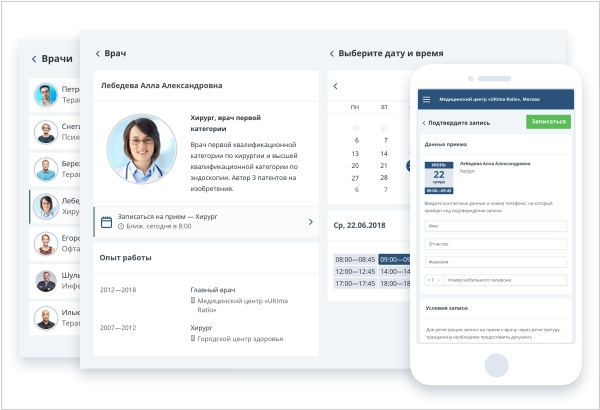
\includegraphics[scale=0.7]{medecs}
		\centering\caption{Интерфейс программы Medesk.}
	\end{figure}
	\subsubsection{MEDODS}
 	{\bf MEDODS} - платформа для организации работы частной медицинской и стоматологической клиники. Позволяет эффективно организовать работу клиники: записывать пациентов на прием, вести электронные медицинские карты, выставлять счета, автоматически формировать договоры, получать сводную статистику работы и многое другое.
 		\\Недостатки:
 	\begin{itemize}
 		\item сложный интерфейс;
 		\item нет возможности вносить свои изменения.
 	\end{itemize}
 	Преимущества:
 	\begin{itemize}
 		\item возможность совершать телефонные вызовы прямо в приложении.
 	\end{itemize}
 	На Рисунке 2 показан внутренний интерфейс программы MEDODS.
 	\clearpage
 	\newpage
 	\begin{figure}[h!]
 		\centering
 		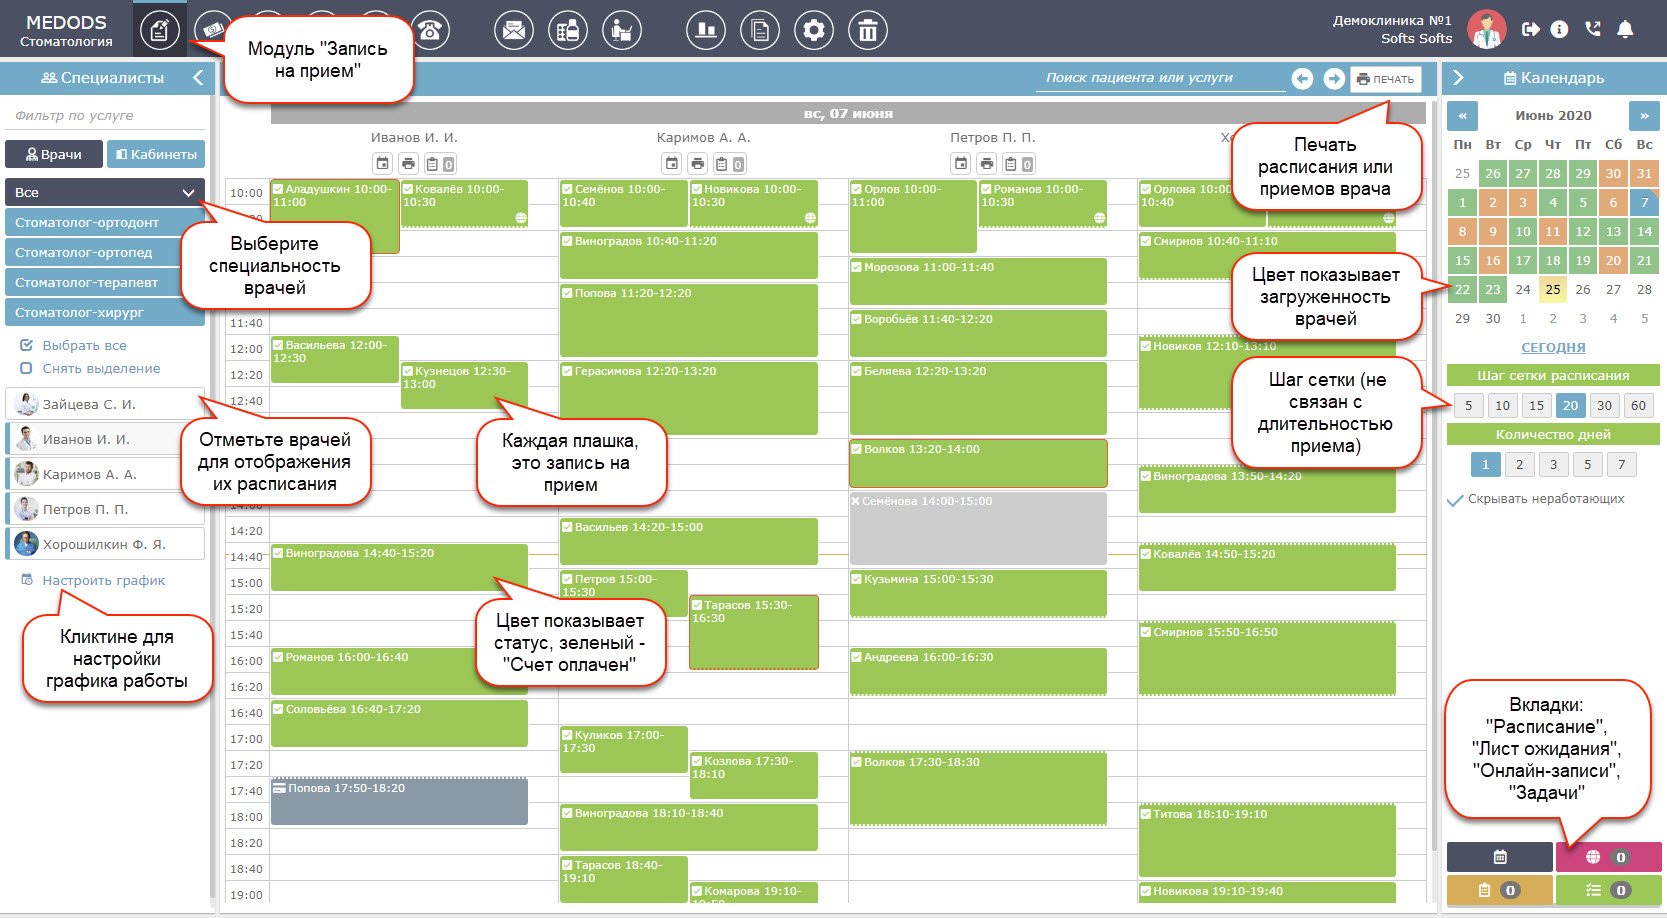
\includegraphics[scale=0.35]{medods}
 		\centering\caption{Интерфейс программы MEDODS.}
 	\end{figure}
 	\subsubsection{Инфоклиника}
 	{\bf Инфоклиника} - полнофункциональная медицинская информационная система: управление поликлиникой, больницей, медицинским центром и сетью медицинских учреждений + SaaS решение для организации сайта электронной регистратуры и личного кабинета пациента клиники.
 	\\Недостатки:
 	\begin{itemize}
 		\item давно не обновлялся;
 		\item очень сложный интерфейс.
 	\end{itemize}
 	Преимущества:
 	\begin{itemize}
 		\item возможность проводить обучения для пользователей;
 		\item беспланый пробный период.
 	\end{itemize}
 	На Рисунке 3 показан внутренний интерфейс программы Инфоклиника.
 	\clearpage
 	\newpage
 	\begin{figure}[h!]
 		\centering
 		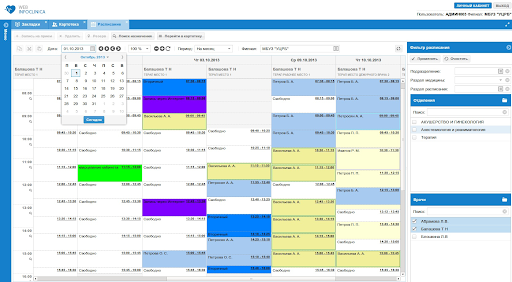
\includegraphics[scale=0.8]{infoklinika}
 		\centering\caption{Интерфейс программы Инфоклиника.}
 	\end{figure}
	\subsubsection{Вывод}
	\hspace*{5mm} Не смотря на то, что существует более чем достаточное количество программного обеспечения для ведения учета в медецинском учреждение, характерными минусами для всего программного обеспечения является высокие требования к аппаратным ресурсам и высокая цена. В своей программе я устраню эти недостатки, сделав его более гибким и доступным для пользователя.
	\subsection{Типы и выбор Баз Данных}
	\hspace*{5mm}Типы баз данных, называемых также моделями БД или семействами БД, представляют собой шаблоны и структуры, используемые для организации данных в системе управления базами данных (СУБД). Выбор типа повлияет на то, какие операции сможет выполнять приложение, как будут представлены данные, на функции СУБД для разработки и рантайма. Разделяют следующие основные виды БД:
	 \begin{enumerate}
	 	\item иерархическая база данных;
	 	\item сетевые базы данных;
	 	\item реляционные базы данных.
	 \end{enumerate}
	\subsubsection{Иерархическая база данных}
	\hspace*{5mm} \textbf{Иерархическая база данных} -  каждый объект при таком хранение информации представляется в виде определенной сущности, то есть, у этой сущности могут быть дочерние элементы, родительские элементы, а у тех дочерних могут быть еще дочерние элементы, но есть один объект, с которого все начинается. Получается своеобразное дерево. Примером иерархической базы данных может быть, документ в формате XML или файловая система компьютера.
	
	 \hspace*{5mm}Следует сказать, что базы данных подобного вида оптимизированы под чтение информации, то есть, базы данных, имеющие иерархическую структуру умеют очень быстро выбирать, запрашиваемую информацию и отдавать ее пользователям. Но такая структура не позволяет столь же быстро перебирать информацию, тут можно привести пример из жизни, компьютер может легко работать с каким-либо конкретным файлом или папкой (которые, по сути являются объектами иерархической структуры) но проверка компьютера антивирусам осуществляется очень долго. Второй пример – реестр Windows.
	 
	\hspace*{5mm}На Рисунке 4 можно увидеть структуру иерархической базы данных, в самом верху находится родитель или корневой элемент, ниже находятся дочерние элементы, элементы, находящиеся на одном уровне называются братьями, ну или соседними элементами. Соответственно чем ниже уровень элемента, тем вложенность этого элемента больше.
	\begin{figure}[h!]
		\centering
		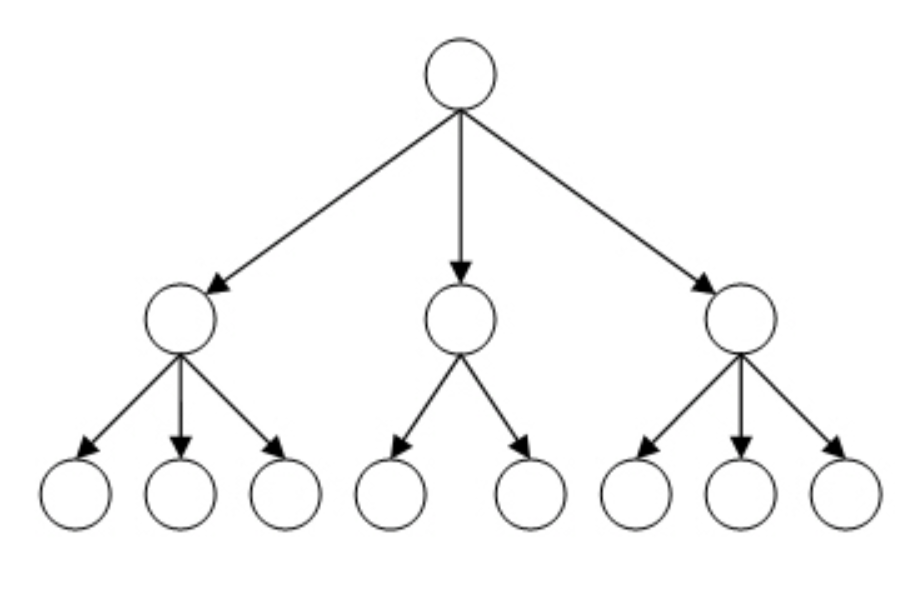
\includegraphics[scale=1]{type1}
		\centering\caption{Структура иерархической базы данных.}
	\end{figure}
	\subsubsection{Сетевые базы данных}
	\hspace*{5mm} \textbf{Сетевые базы данных} - являются своеобразной модификацией иерархических баз данных. Если обратить внимание на Рисунок 4, можно заметить, что к каждому нижнему элементу идет только одна стрелочка от верхнего элемента. То есть у иерархических баз данных у каждого дочернего элемента может быть только один потомок. Сетевые базы данных отличаются от иерархических тем, что у дочернего элемента может быть несколько предков, то есть, элементов стоящих выше него. Для большей наглядности и понимания структуры сетевых баз можно увидель на Рисунке 5.
	\clearpage
	\newpage
	\begin{figure}[h!]
		\centering
		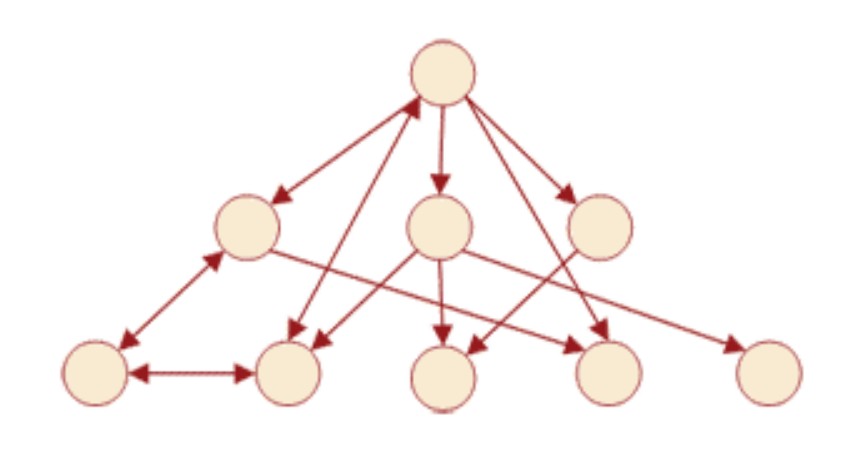
\includegraphics[scale=1.2]{type2}
		\centering\caption{Структура сетевой базы данных.}
	\end{figure}
	\hspace*{5mm}Стоит заметить, что сетевые базы данных обладают примерно теми же характеристиками, что и иерархические базы данных.
	\subsubsection{Реляционные базы данных}
	\hspace*{5mm} Главной особенностью \textbf{реляционных баз данных} является, то, что объекты внутри таких баз данных хранятся в виде набора двумерных таблиц. То есть, таблица состоит из набора столбцов, в котором может указываться: название, тип данных(дата, число, строка, текст и т.д.). Еще одной важной особенность реляционных БД является, то, что число столбцов фиксировано, то есть, структура базы данных известна заранее, а вот число строк или рядов в реляционных базах данных ничем не ограничено. Тем самым получается, что строки в реляционных базах данных и есть объекты, которые хранятся в базе данных.
	\\ \hspace*{5mm} Самой трудной задачей при работе с реляционными базами данных, является проектирование структуры баз данных. Проектирование структуры базы данных, заключается не только в том, чтобы создать таблицу и указать тип данных и наименование столбцов. На самом деле проектирование – это самый сложный этап при работе с базами данных. Потому что мощности ваших компьютеров ограничены. Пока данных мало, мало таблиц и строк в этих таблицах, машина будет их обрабатывать очень и очень быстро. Но, со временем количество информации будет увеличиваться, и мы получим замедление, которое будет увеличиваться, поскольку машине необходимо время на обработку тех или иных запросов(обработка информации).
	\clearpage
	\newpage
	\begin{figure}[h!]
		\centering
		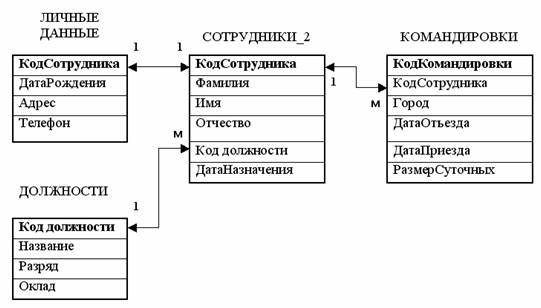
\includegraphics[scale=1]{type3}
		\centering\caption{Структура реляционной базы данных.}
	\end{figure}
	\subsubsection{Вывод}
	\hspace*{5mm} Не смотря на то, что существует разные типы баз данных, в данной работе была выбрана реляционная модель. Эта модель была выбрана за следующие достоинства:
	\begin{enumerate}
		\item простота и доступность для понимания пользователем. Единственной используемой информационной конструкцией является "таблица";
		\item строгие правила проектирования, базирующиеся на математическом аппарате;
		\item полная независимость данных. Изменения в прикладной программе при изменении реляционной БД минимальны;
		\item для организации запросов и написания прикладного ПО нет необходимости знать конкретную организацию БД во внешней памяти. 
	\end{enumerate}
%\end{flushleft}
\clearpage
\newpage
\section{Конструкторская часть}
%\begin{flushleft}
	 \subsection{Разработка структуры БД}
	 На Рисунке 7 показана ER-диаграмма, описывающая концептуальные схемы предметной области. База данных состоит из 5 таблиц: 
	 \begin{enumerate}
	 	\item patients;
	 	\item records;
	 	\item doctors;
	 	\item services;
	 	\item discharge.
	 \end{enumerate}
 	В таблице Patients хранится уникальная информация о пациенте, а именно его имя, дата рождения и номер телефона. Каждый пациент может иметь неограниченное число посещений у врача, в следствие чего, создана таблица Records, которая направлена на хранение информации о каждом приеме у врача. Эта модель тесно связана с таблицами Doctors, Services, Discharge.
	\begin{figure}[h!]
		\centering
		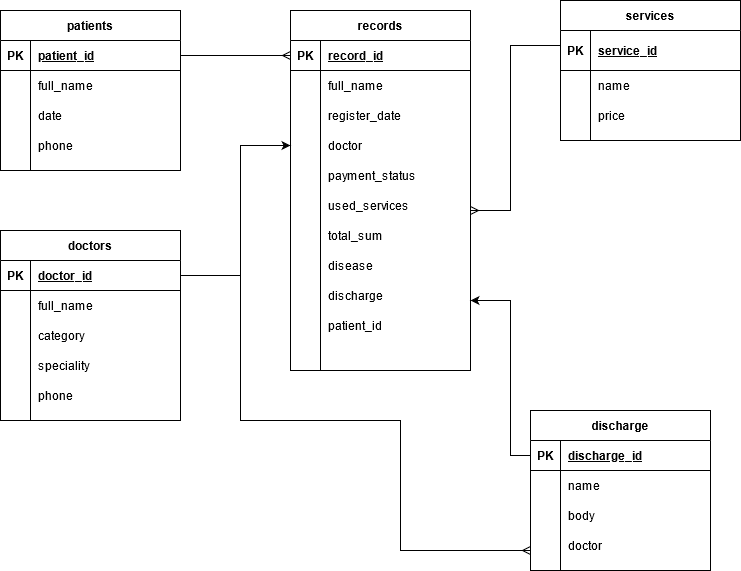
\includegraphics[scale=0.6]{er-diagram}
		\centering\caption{ER-модель структуры БД}
	\end{figure}
	\clearpage
	\newpage
	\subsection{Use-Case диаграмма БД с выделением акторов}
	На Рисунке 8 показана Use-Case диаграмма БД с выделением акторов, описывающая струкутру и логику данного ПО. На рисунке видно, как выделено 3 актора: Регистратура, Врач, Пациент. 
	\begin{figure}[h!]
		\centering
		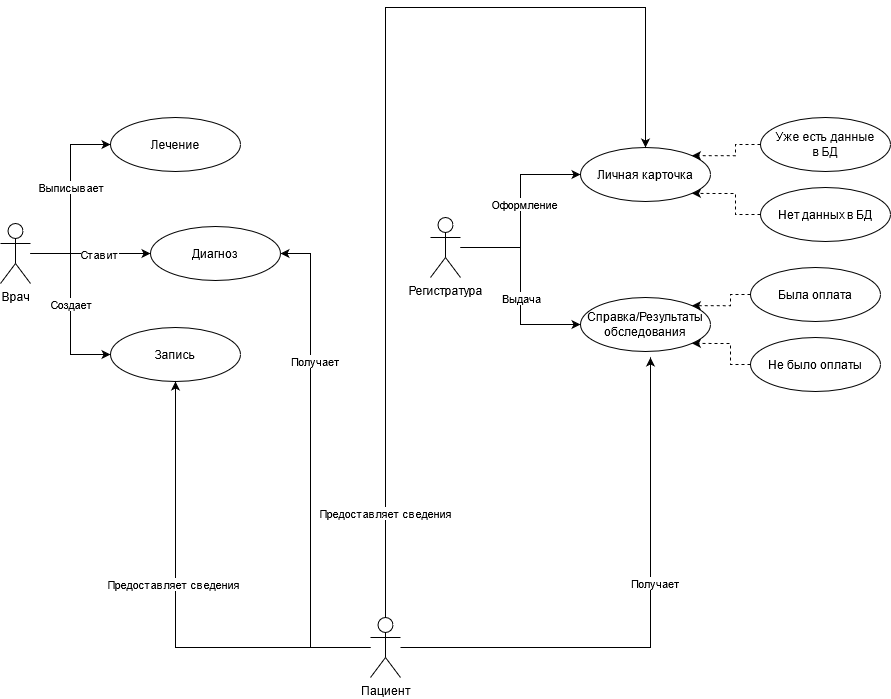
\includegraphics[scale=0.5]{use-case}
		\centering\caption{Use-Case диаграмма БД с выделением акторов}
	\end{figure}
	\subsection{IDEF0 диаграмма для функции авторизации}
	На Рисунке 9 показана IDEF0 диаграмма Функции авторизации. 
	\clearpage
	\newpage
	\begin{figure}[h!]
		\centering
		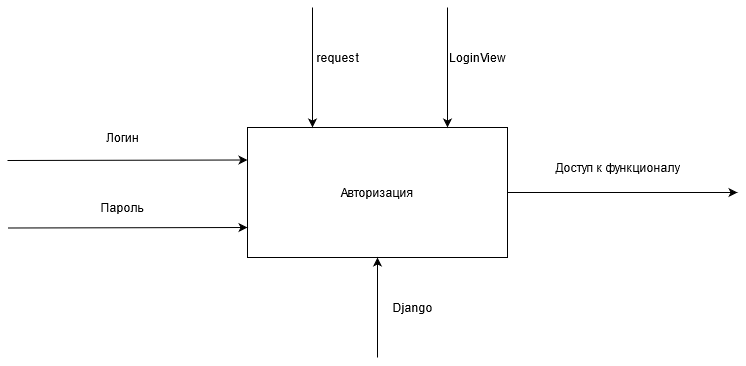
\includegraphics[scale=0.5]{idef02}
		\centering\caption{IDEF0 диаграмма для функции авторизации}
	\end{figure}
	\subsection{IDEF0 диаграмма для функции скачинавания рецепта на лечение}
	На Рисунке 10 показана IDEF0 диаграмма для функции скачинавания рецепта на лечение. Стоит отметь что данная функция достпна только тогда, когда пациент произведет оплату за оказанные ему услуги. Данный статус может быть отмечен только регистратором или кассиром. У врачей данная функция отсутствует, ввиду того, чтобы решить проблему с финансовостью.
	
	\begin{figure}[h!]
		\centering
		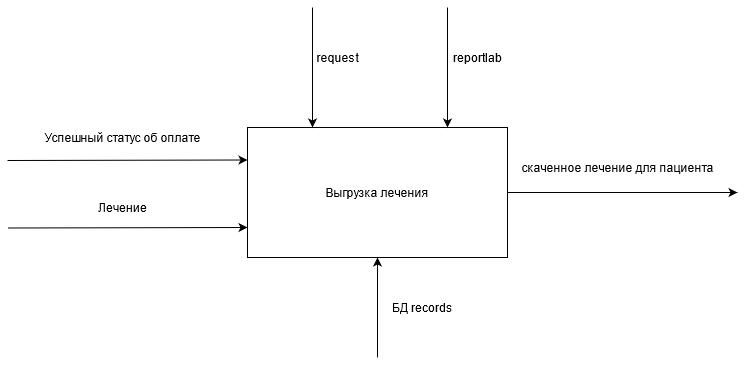
\includegraphics[scale=0.5]{idef01}
		\centering\caption{IDEF0 диаграмма для функции скачинавания рецепта на лечение}
	\end{figure}
	\subsection{Вывод из конструкторской части}
	\hspace*{5mm} В данном разделе были представлены схемы и диаграммы представляющую структуру БД, а также описывающую логику ее работы. Так же были показаны диаграммы некоторых основных функций ПО.	 
%\end{flushleft}
\clearpage
\newpage
\section{Технологическая часть}
%\begin{flushleft}
	\hspace*{5mm} В данном разделе будут рассмотрены требования к программному обеспечению, средства реализации.

	\subsection{Архитектура программного обеспечения}
	\hspace*{5mm} В соответствии с техническим заданием будущее приложение должно иметь трехзвенную систему: веб-приложение(представление), базу данных(модель) и логику на серверной части(контроллер). Основная цель применения этой концепции состоит в отделении бизнес-логики(модели) от её визуализации. За счёт такого разделения повышается возможность повторного использования кода.
	\subsection{Выбор среды и языка разработки серверной части}
	При выборе языка будем руководствоваться следующими факторами:
	\begin{enumerate}
		\item платформ независимый;
		\item динамический;
		\item высокоуровневый;
		\item многопоточный.
	\end{enumerate}
	\hspace*{5mm} Под динамическим в данном случае понимается, что программа может выполнять обширное количество задач во время обработки информации, которая может быть использовано для проверки и разрешения доступа к объектам на время выполнения. 
	\\ \hspace*{5mm} Всем этим критериям удовлетворяет язык Python3. Основным достоинством является то, что с помощью данного языка можно «разбить» реализацию: интерфейс, работу с файлами и элементами формы организовать с помощью встроенных средств. 
	\\ \hspace*{5mm} При выборе среды разработки рассматриваются и другие возможные среды, которые помогут автоматизировать процесс разработки. Для разработки данной программы необходимо обеспечение средой следующих возможностей: 
	\begin{enumerate}
		\item удобные инструменты для отладки и поиска ошибок, в случае их возникновения;
		\item разработка более гибкой и надежной программы путем обработки различных исключительных ситуаций, возникающих в результате некорректной работы программы;
		\item использование всплывающих подсказок во время написания кода программы, что обеспечивает значительное экономию времени и повышения уровня продуктивности.
	\end{enumerate}
	\hspace*{5mm} Среда разработки PyCharm\cite{pycharm} поддерживает все эти возможности, а также многие другие, такие как: 
	\begin{enumerate}
		\item инструменты для запуска тестов и анализа покрытия кода, включая поддержку всех популярных фреймворков для тестирования;
		\item инструменты для работы с базами данных и SQL файлами, включая удобный клиент и редактор для схемы базы данных;
		\item окно классов для перехода по исходному коду по типам, а не файлам;
		\item обозреватель документов для просмотра и поиска документации по продуктам на локальном компьютере или в Интернете;
		\item умное автодополнение, инструменты для анализа качества кода, удобная навигация, расширенные рефакторинги и форматирование;
		\item окно Свойства для настройки свойств и событий элементов управления в пользовательском интерфейсе.
	\end{enumerate}
	\hspace*{5mm} Среду разработки PyCharm стоит рассматривать как интеллектуальную среду разработки, понимающую код. В процессе его написания программистом она занимается построением синтаксического дерева, определением особенностей размещенных ссылок, анализом возможных путей исполнения операторов и передачи данных.
	\subsection{Используемые инструменты и технологии веб-приложения}
	\hspace*{5mm}Для облегчения разработки веб-приложения нужно использовать фреймворки, которые являются набором шаблонов или заготовок, облегчающий разработку и объединение разных модулей программного проекта. 
	\\ \hspace*{5mm} Одними из популярных фреймворков являются PHP-фреймворки Zend Framework и Symfony или Django\cite{djangoproject}, написанный на Python. 
	\\ \hspace*{5mm} Основным критерием выбора является язык разработки серверной части, который должен корректно взаимодействовать с Фреймворком.  
	\\ \hspace*{5mm} Анализируя различные инструменты, для разработки веб-приложения был выбран универсальный фреймворк с открытым исходным кодом Django написанный на Python3\cite{python}. Для написания лицевой части приложения были использованы HTML\cite{html}, CSS\cite{css}, JavaScript, Bootstrap\cite{bootstrap}. В качестве СУБД была выбрана PostgreSQL\cite{postgres}.
	\subsection{Реализация}
	\hspace*{5mm} Для работы с базой данных Django\cite{djangoproject} использует собственную технологию программирования, в которой модель данных описывается классами Python, и по ней генерируется схема базы данных. В качестве среды разработки выбран редактор PyCharm. 
	\\ \hspace*{5mm} В терминале PyCharm с помощью команды python manage.py runserver запускается сервер, выделяется адрес для localhost. В данном случае был выделен адрес 127.0.0.1:8000. 
	
	\subsection{Интерфейс программы}
	\hspace*{5mm} Ниже представлен интерфейс полученного веб-приложения. 
	\clearpage
	\newpage
	\begin{figure}[t!]
		\centering
		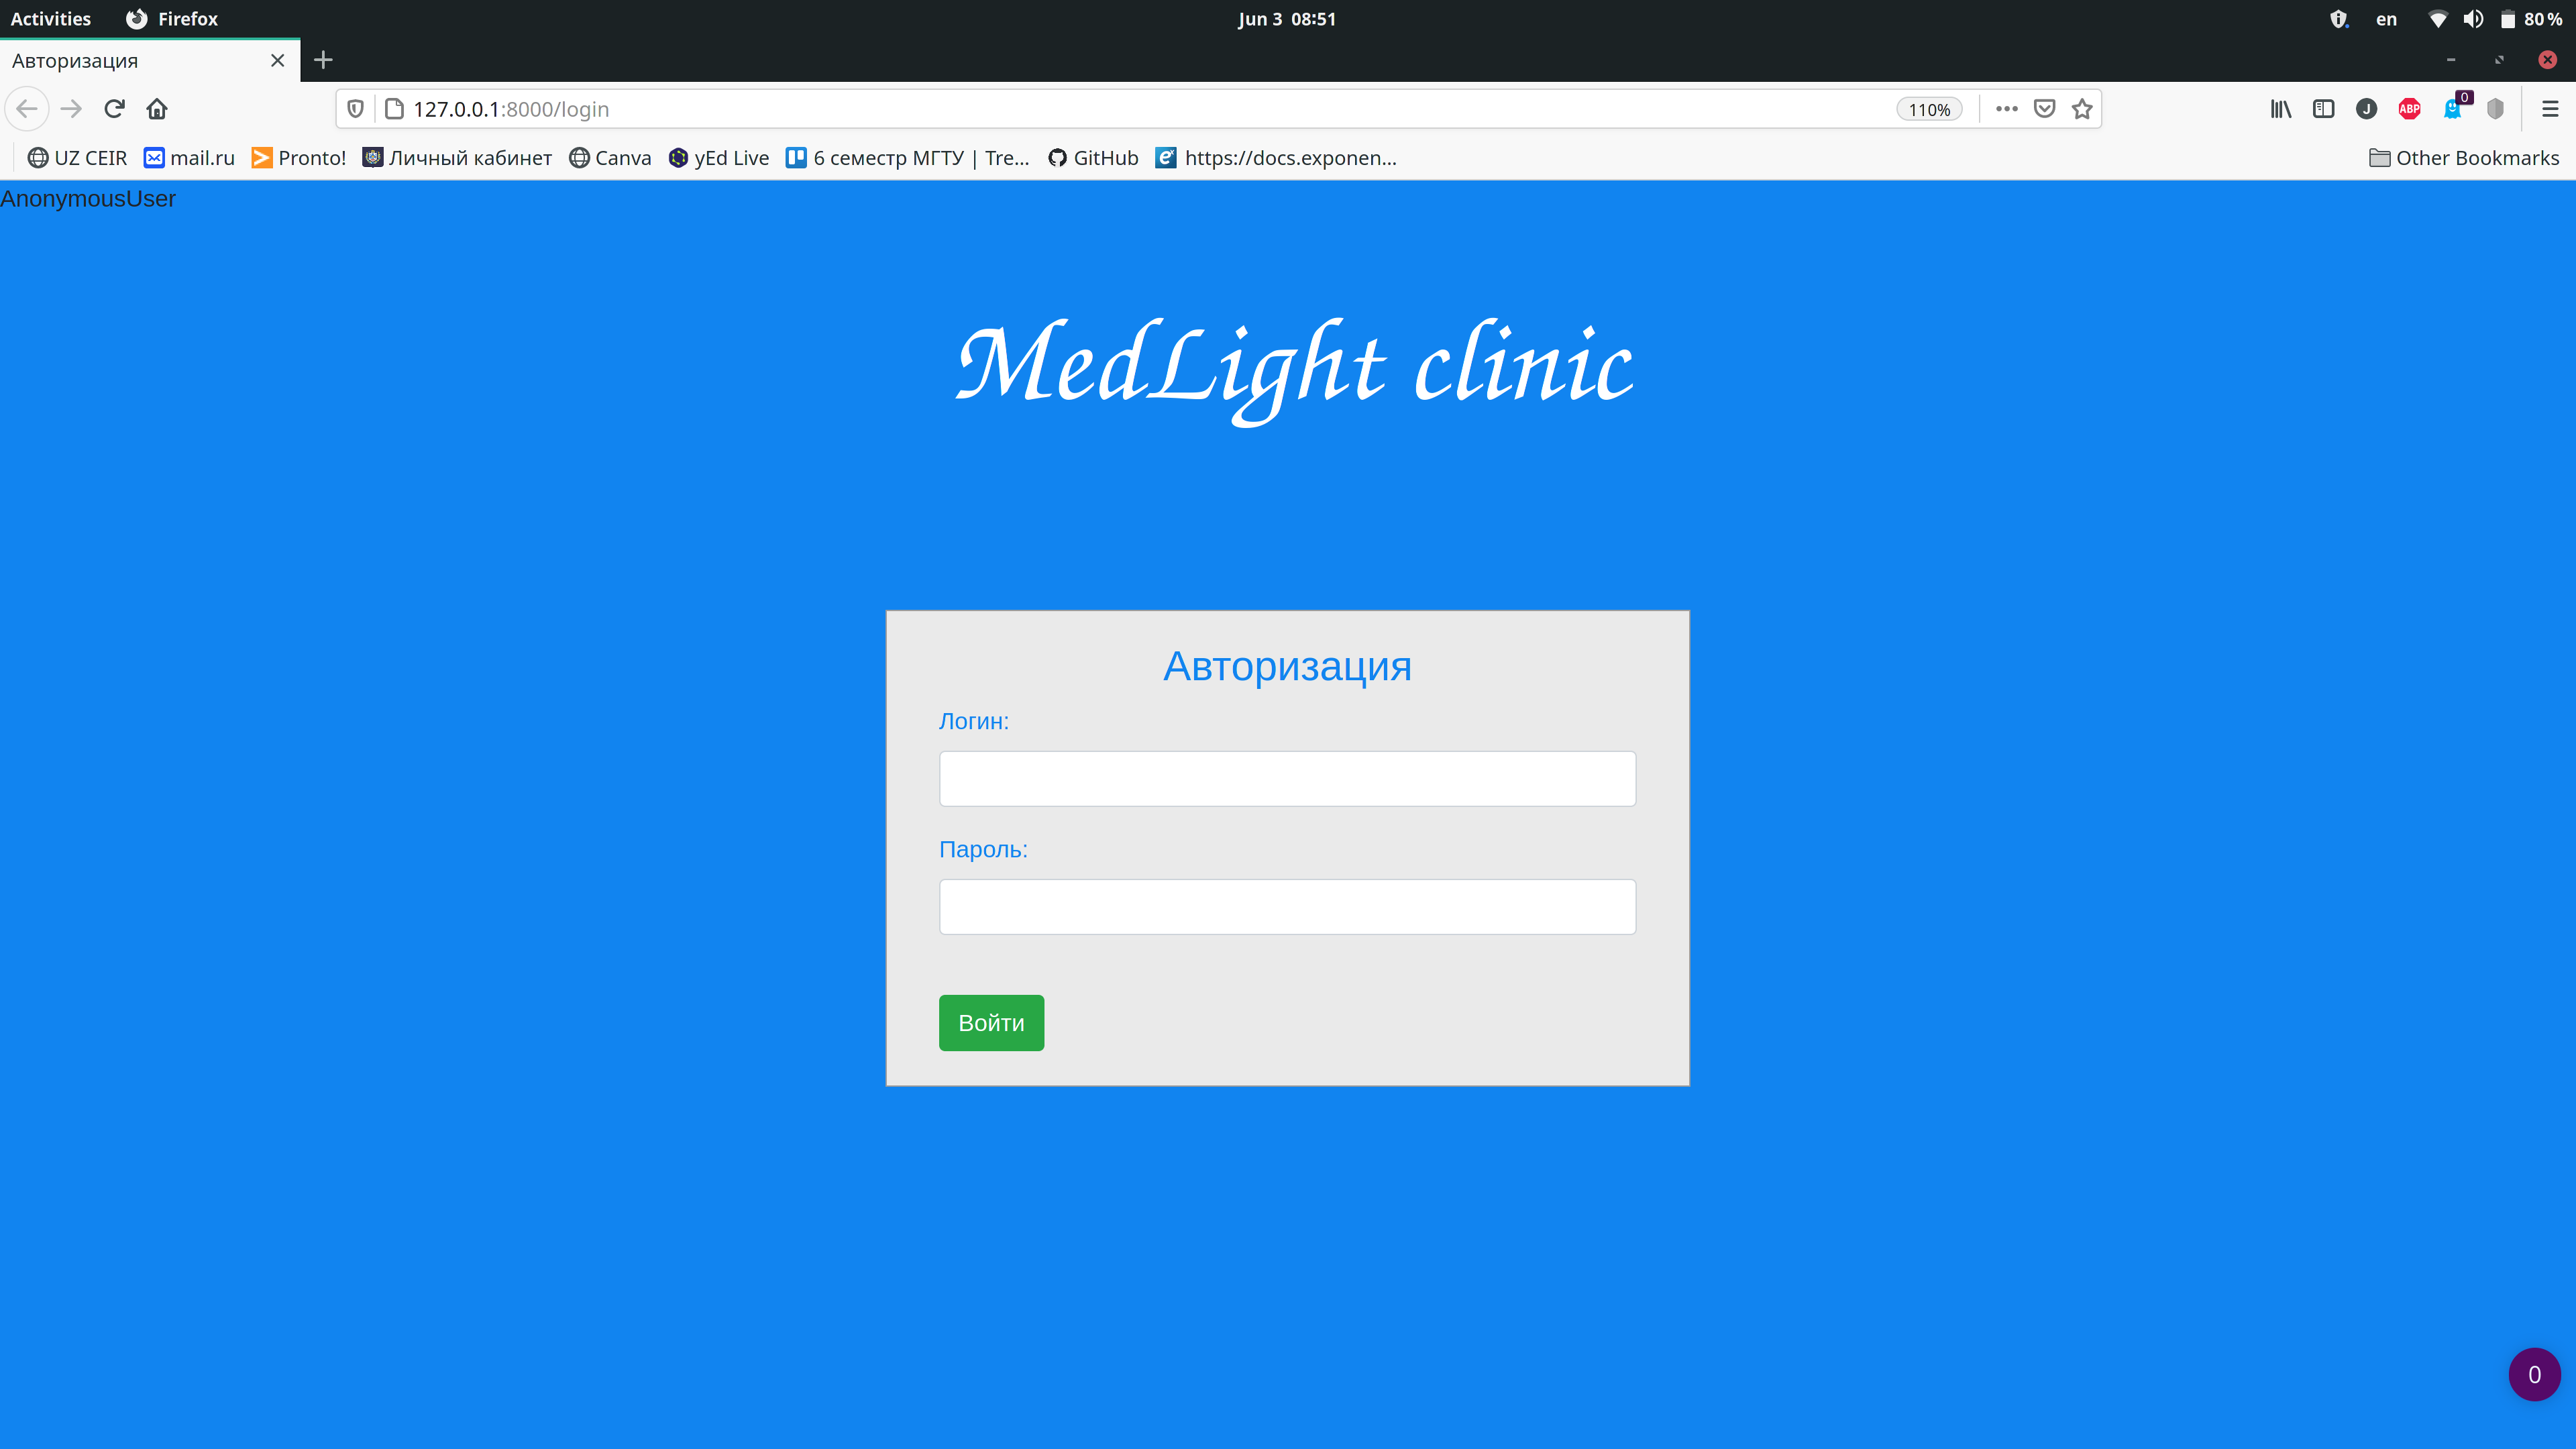
\includegraphics[scale=0.12]{auth}
		\centering\caption{Интерфейс модуля <<Авторизация>>}
	\end{figure}
	\hspace*{5mm} На рисунке 11 показано модуль \textbf{Авторизации}, где пользователю необходимо ввести логин и пароль от системы. В случае успеха, пользователю будет доступен функционал в соответствии с его ролью в приложение.
	 \begin{figure}[h!]
	 	\centering
	 	
\includegraphics[scale=0.12]{main}
	 	\centering\caption{Интерфейс главного меню}
	 \end{figure}
 	\clearpage
 	\newpage
 		\begin{figure}[h!]
 			\centering
 			
\includegraphics[scale=0.12]{menu}
 			\centering\caption{Содержание меню}
 		\end{figure}
 	\begin{figure}[h!]
 		\centering
 		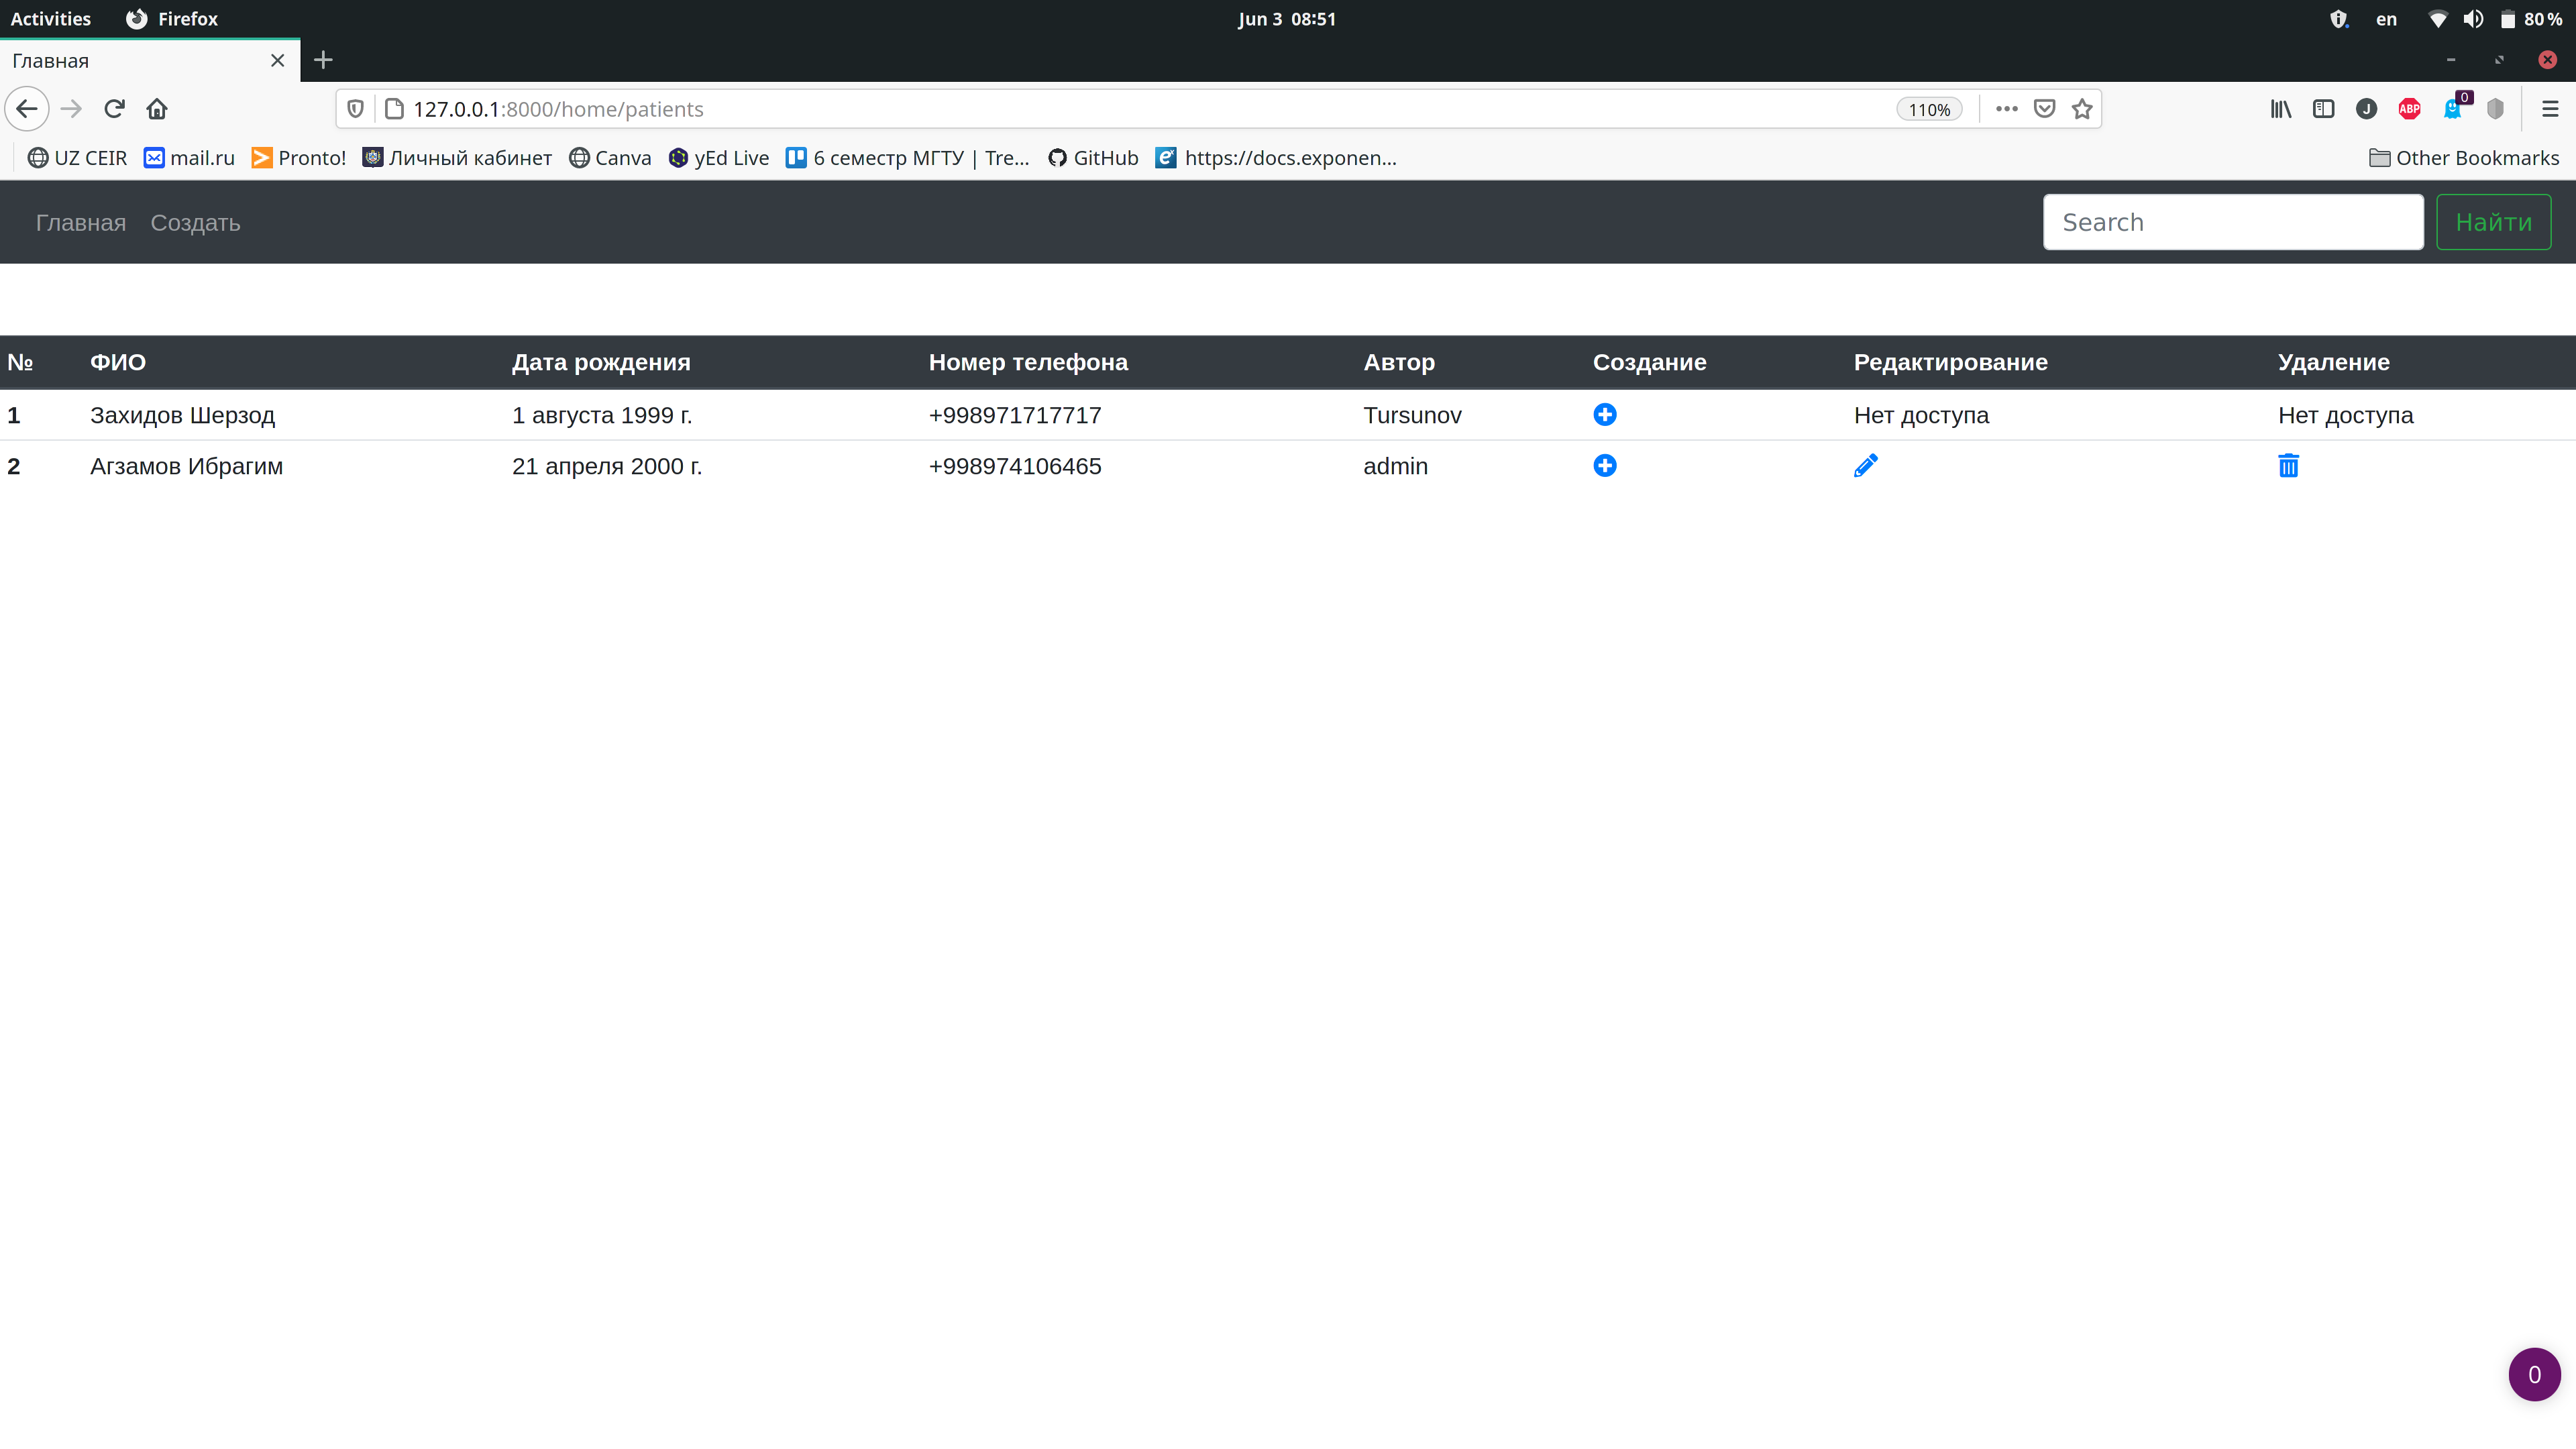
\includegraphics[scale=0.12]{patients}
 		\centering\caption{Страница <<Пациенты>>}
 	\end{figure}
 	\hspace*{5mm} На этой странице, пользователю будет доступен список всех пациентов. Для каждого пациента, пользователь может созадть запись у врача(Рисунок 15). Функционал удаления и измения данных о пациенте доступен только Админестратору и тем кто эти записи создал. Также на странице имеется возможность сделать поиск. Поиск работает по всем ключевым полям.
 	\clearpage
 	\newpage
 	\begin{figure}[h!]
 		\centering
 		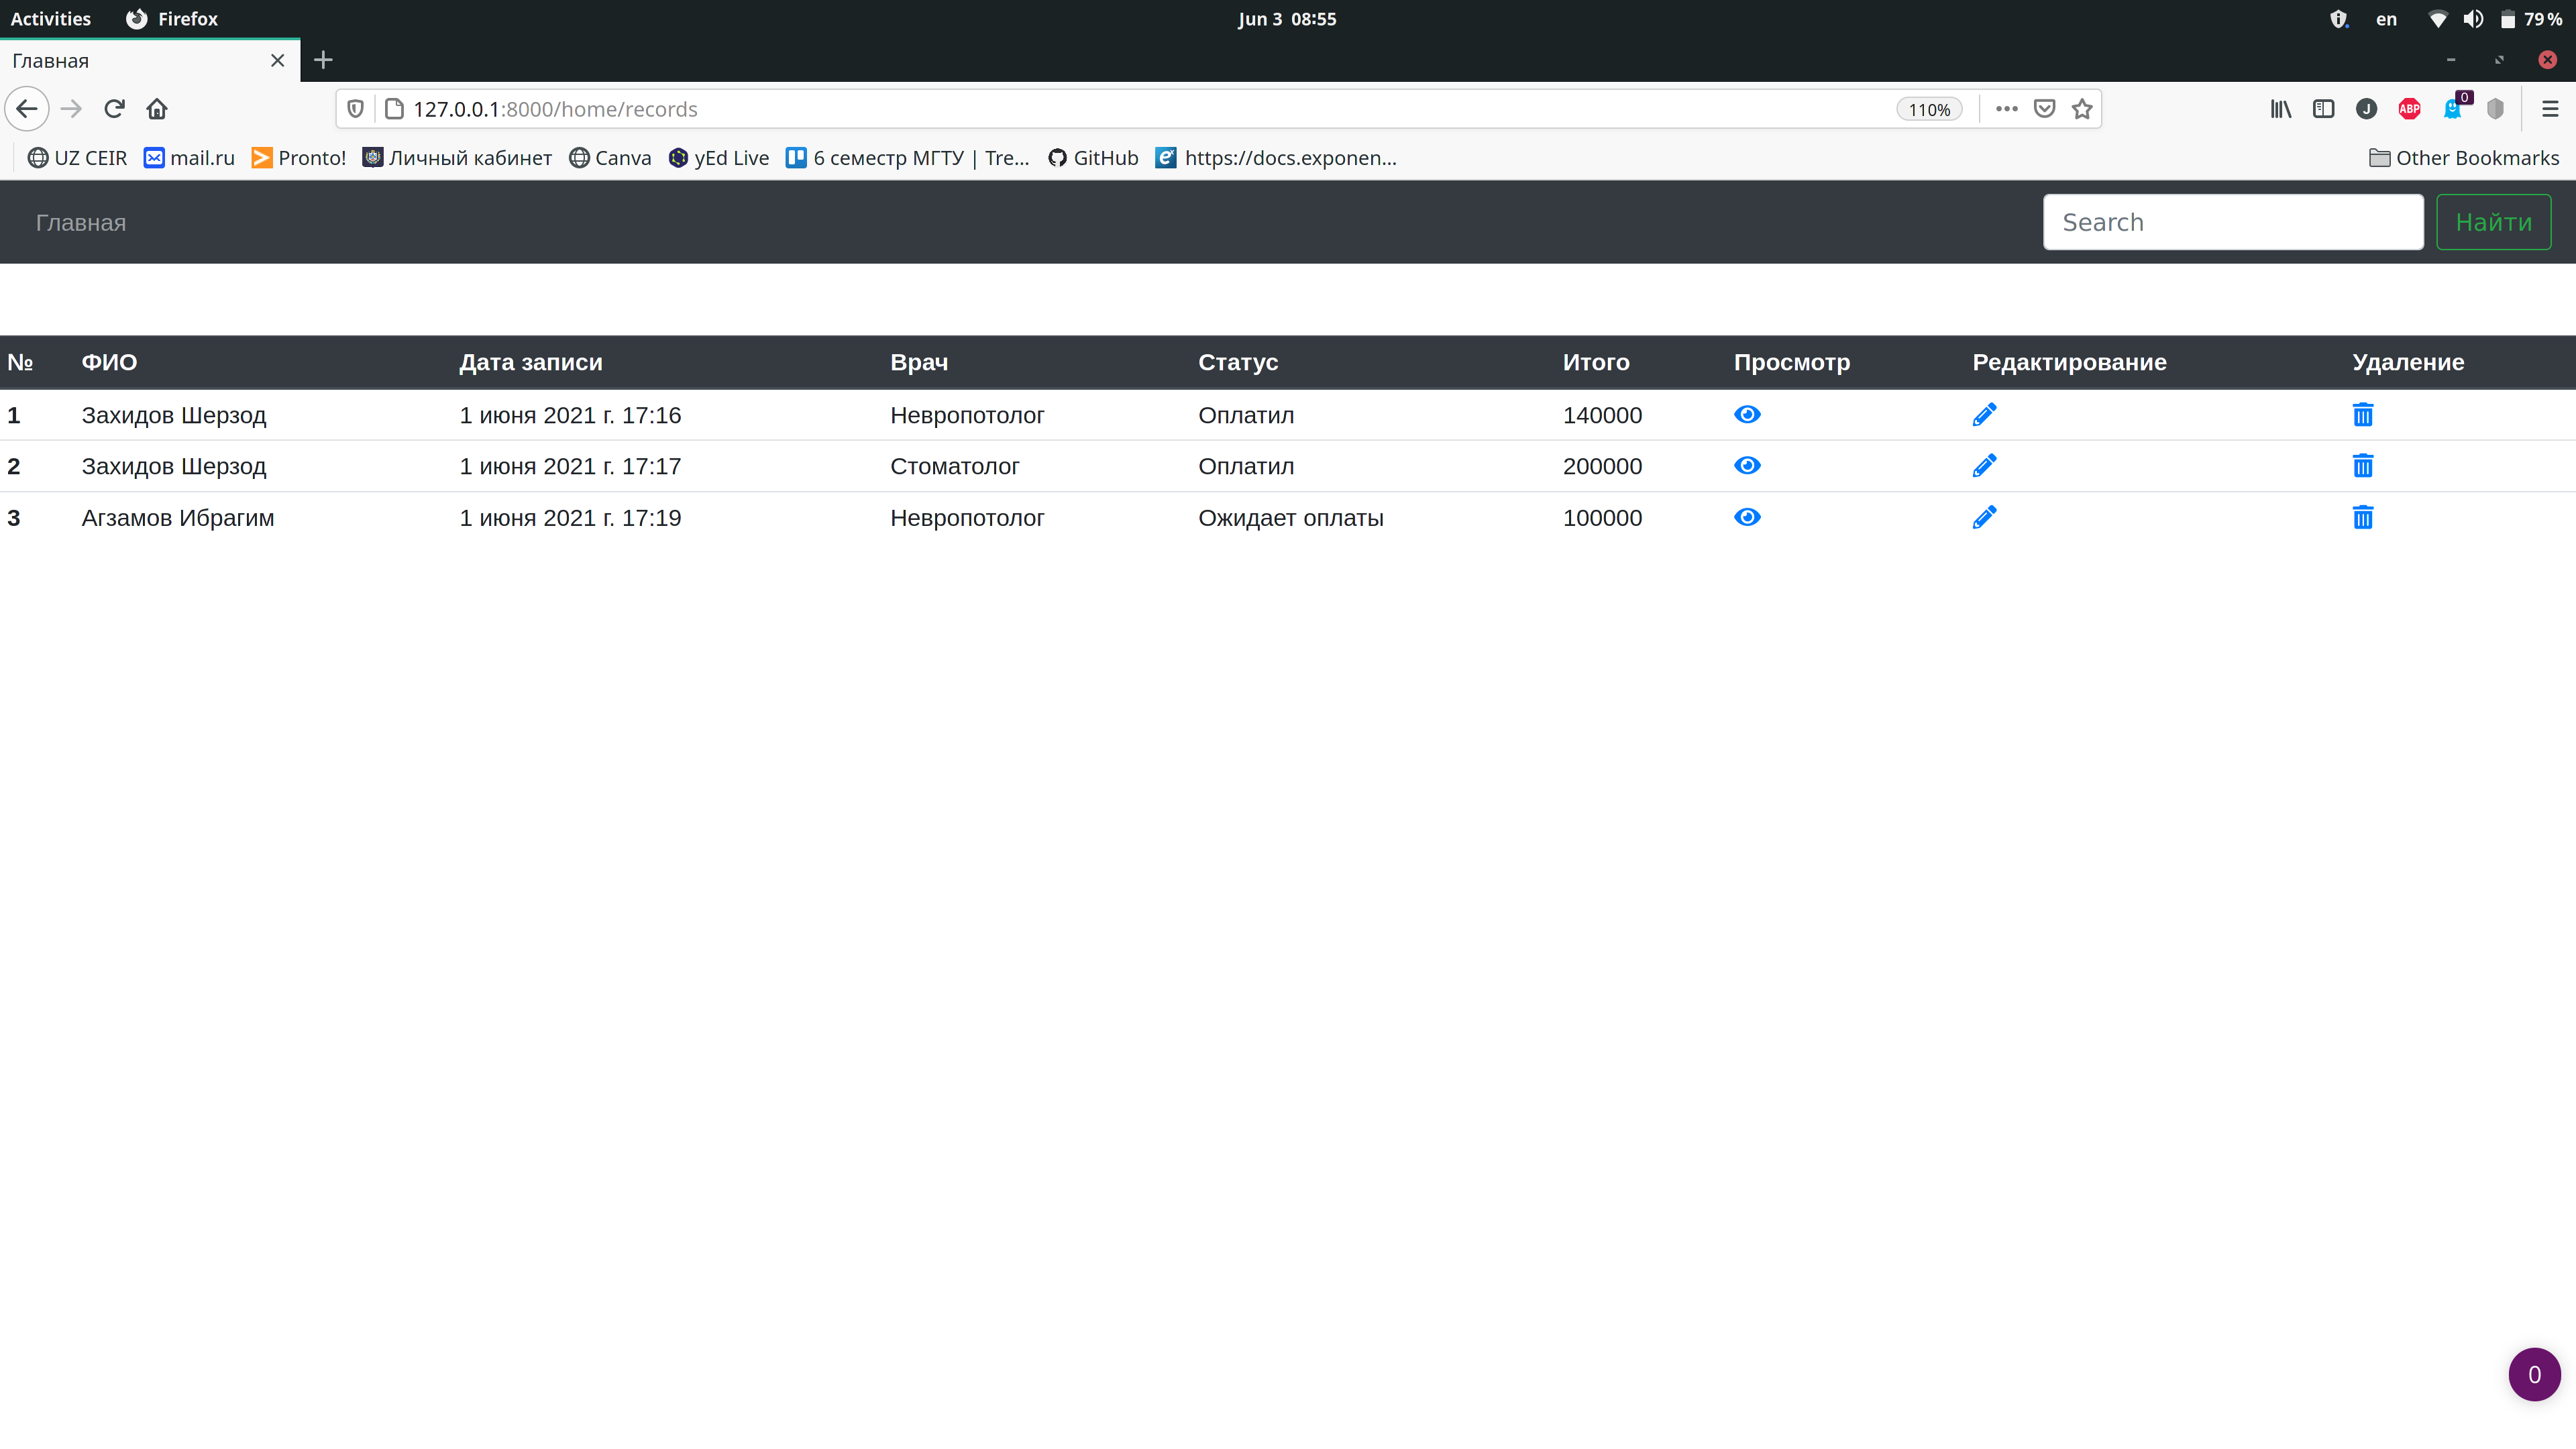
\includegraphics[scale=0.12]{records}
 		\centering\caption{Страница <<Записи>>}
 	\end{figure} 
 	\hspace*{5mm} На этой странице, пользователю будет доступен список всех записей. Для каждого пациента, пользователь может просмотреть, обновить или удалить запись. Пользователю будет доступен функционал <<Скачивания>> рецепта на лечение, только в том случае, если была произведена оплата.
 	\begin{figure}[h!]
 		\centering
 		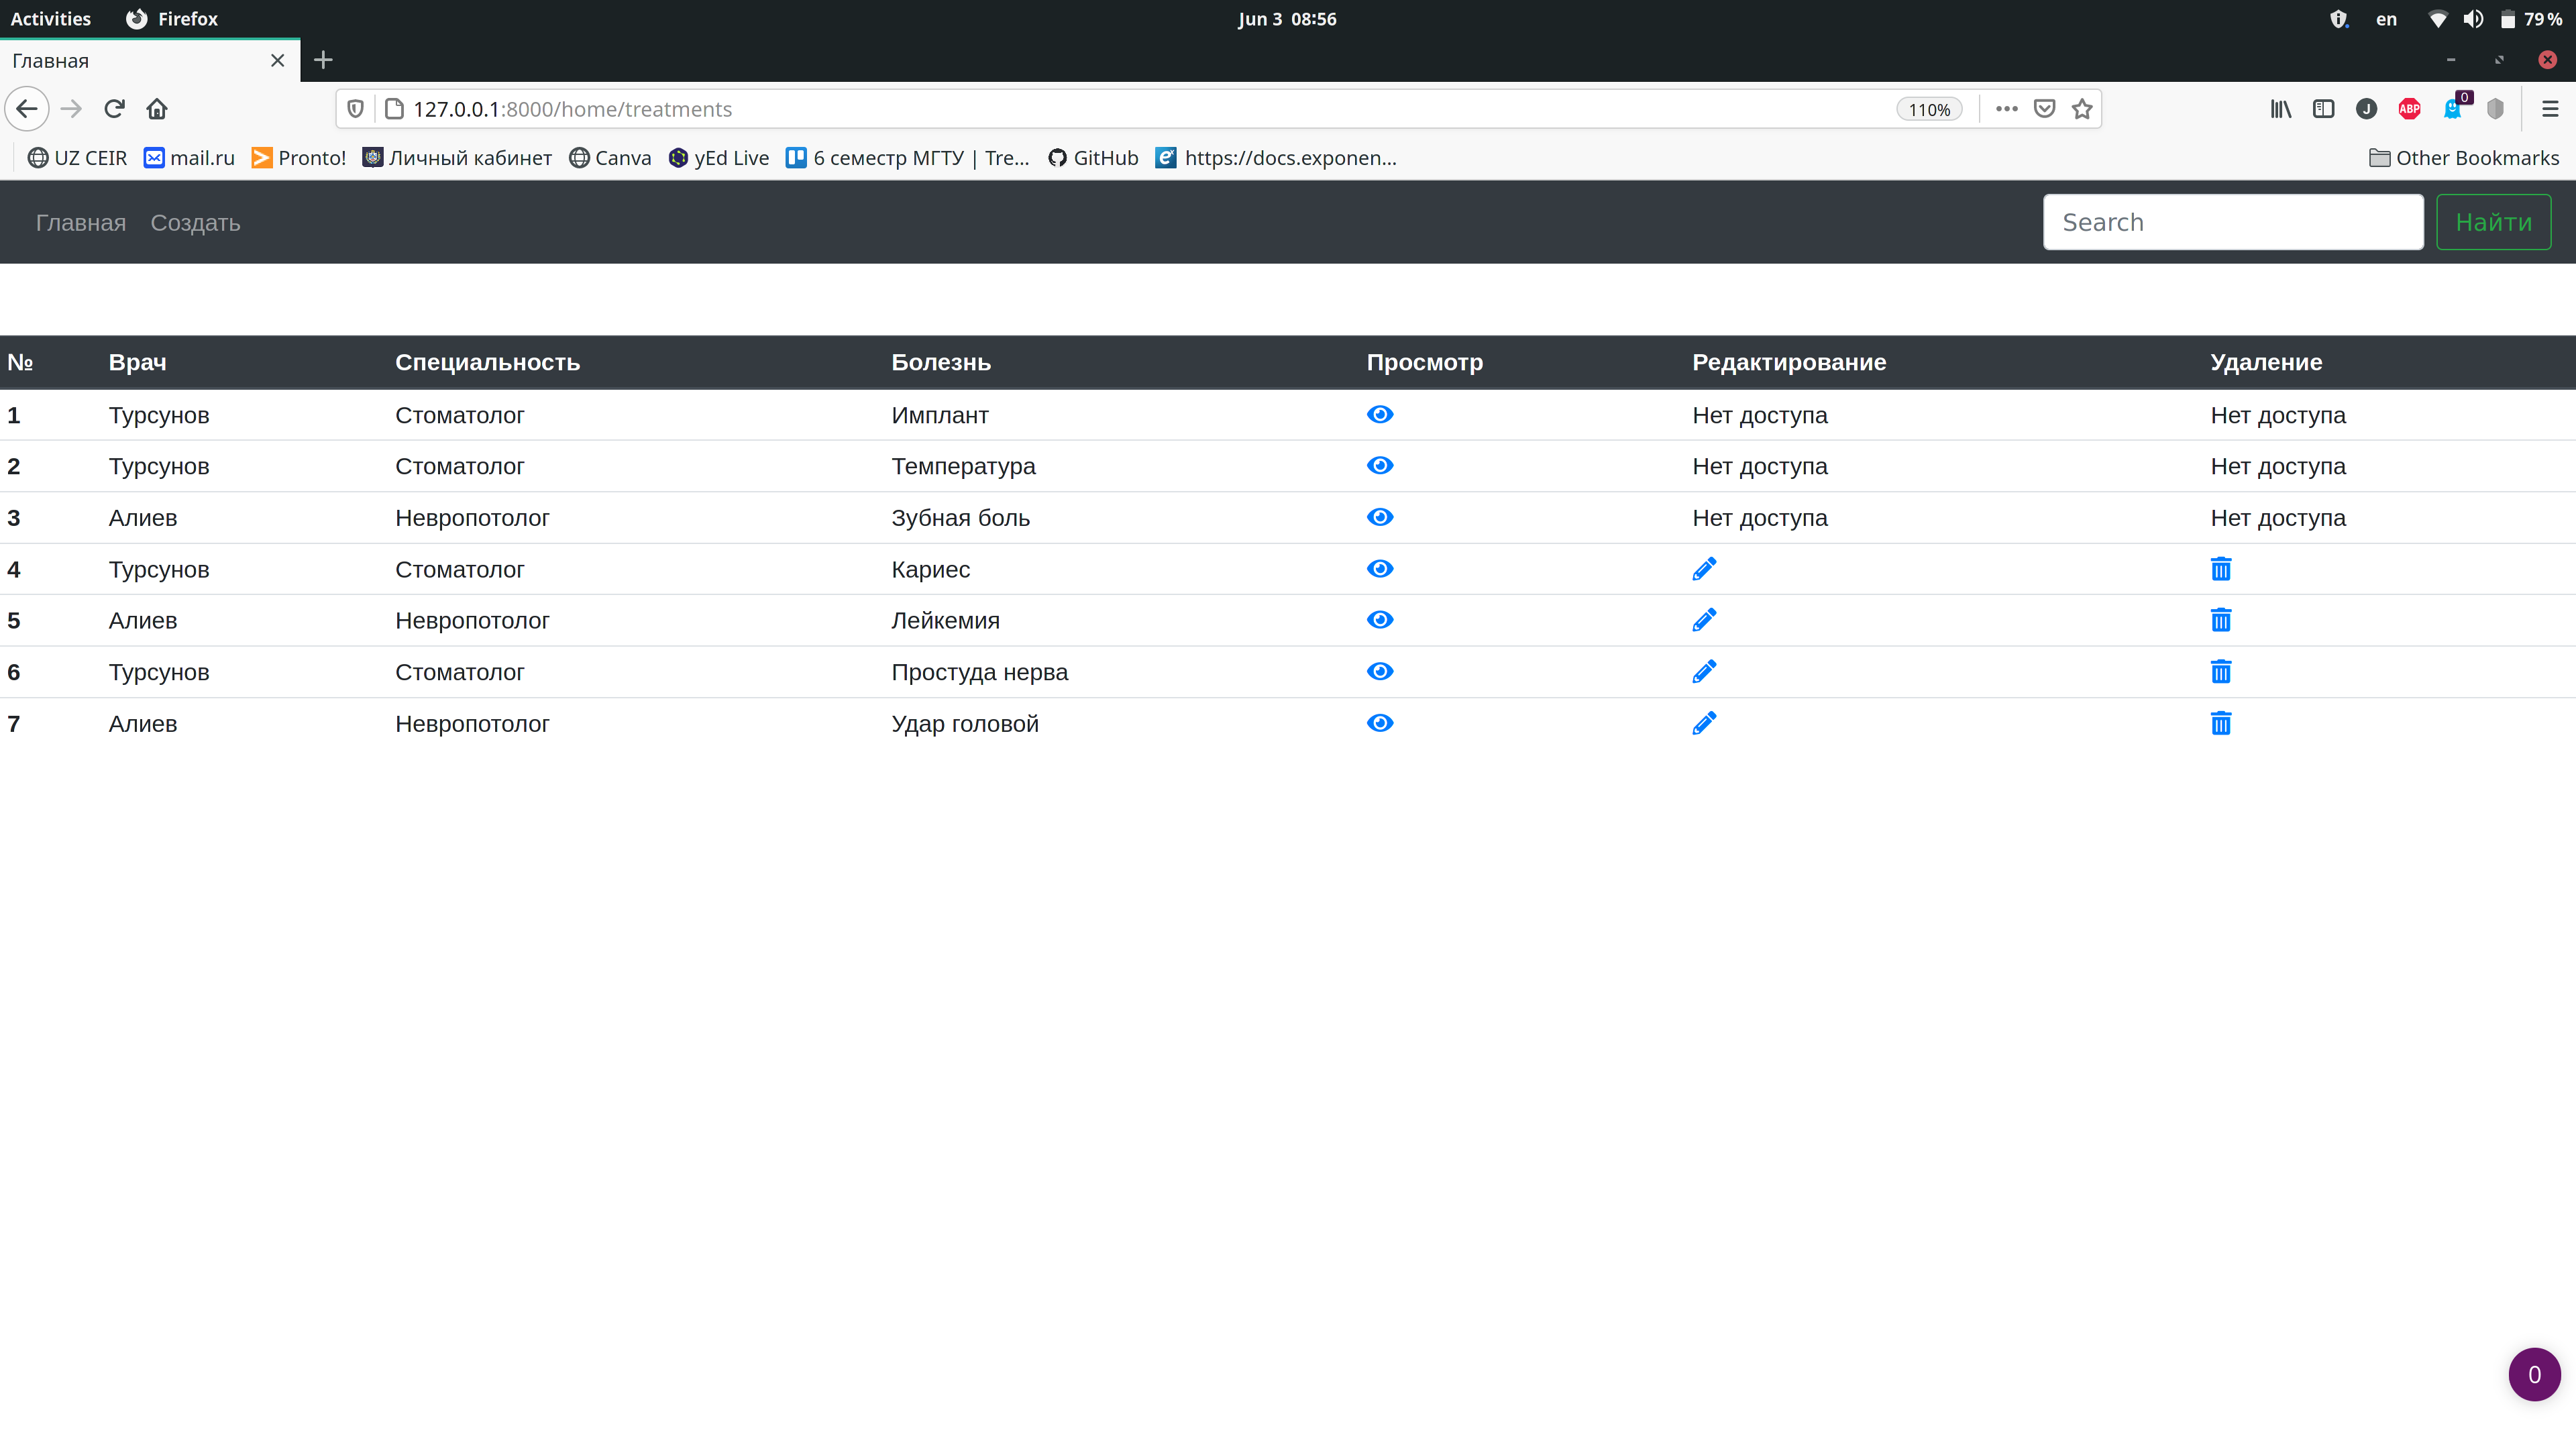
\includegraphics[scale=0.12]{discharges}
 		\centering\caption{Страница <<Стандартные лечения>>}
 	\end{figure}
 	\clearpage
 	\newpage
 	\hspace*{5mm} На текущей странице пользователь может создать для себя готовое лечение, для его использования при созадние записи для пациента. Этот функционал облегчает работу врачей, так как иногда приходится повторно записывать одно и то же лечение несколько раз, пациентам с одинаковым диагнозом. 
 	\begin{figure}[h!]
 		\centering
 		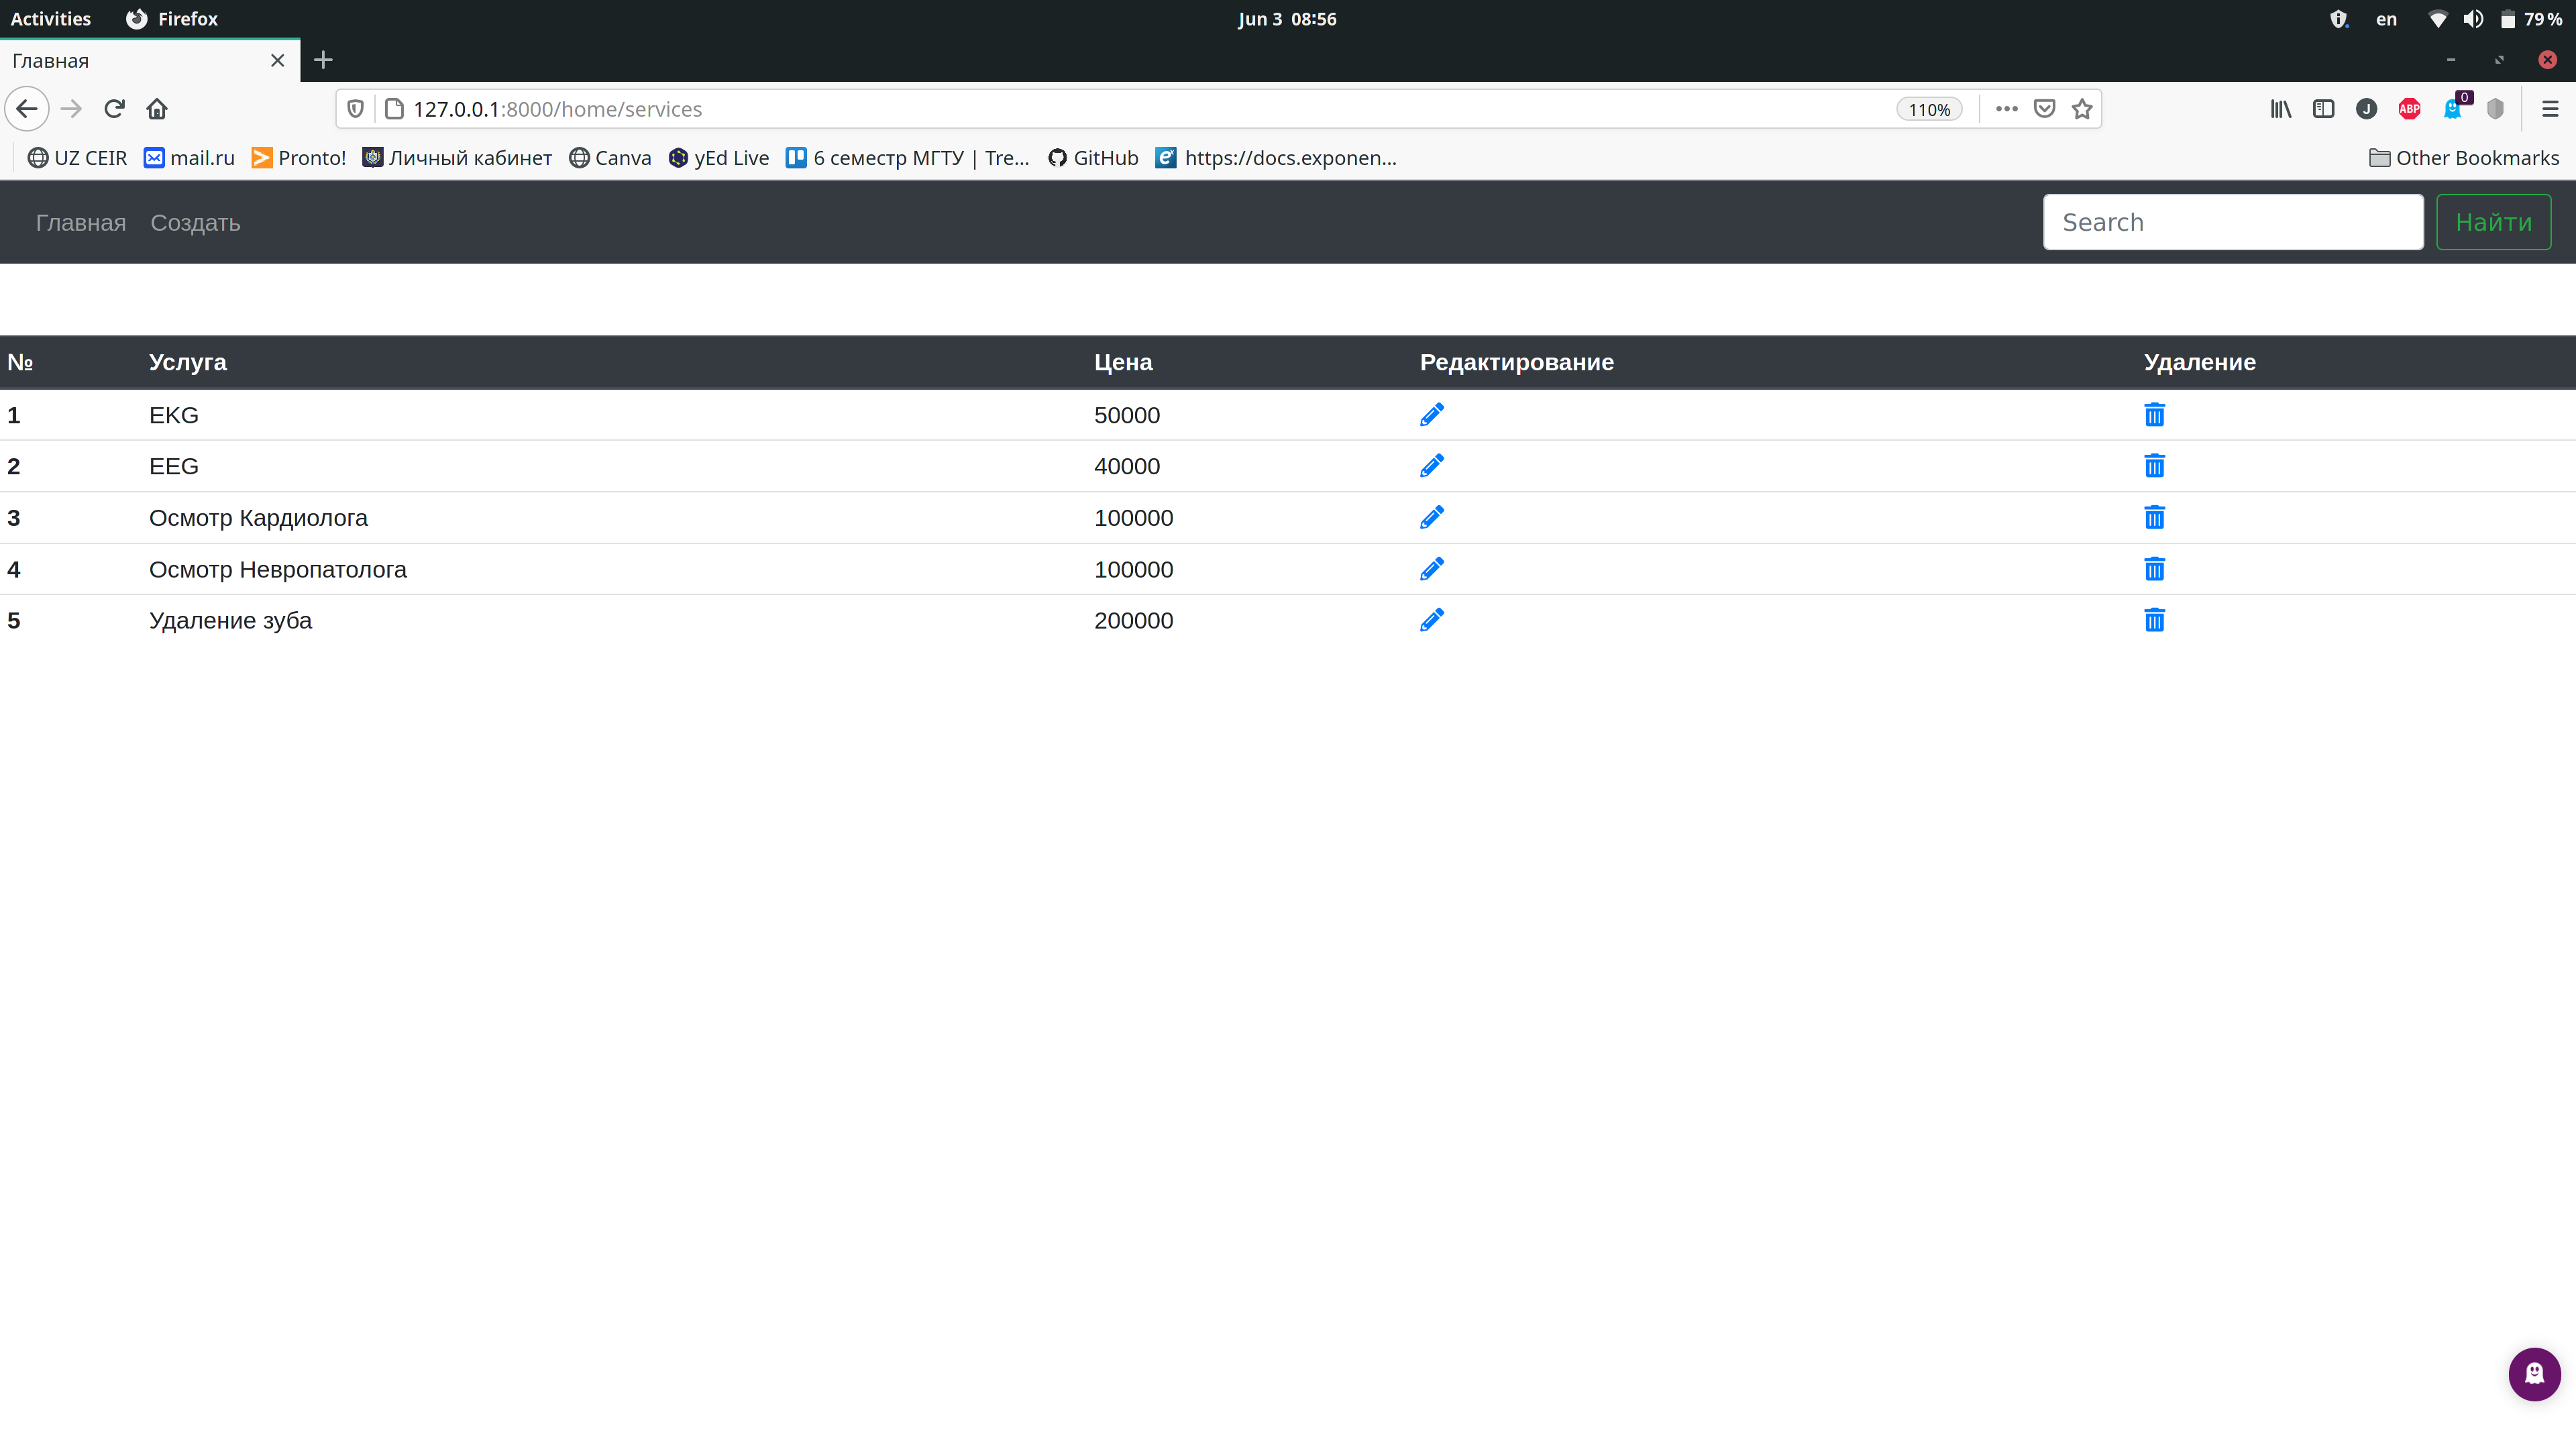
\includegraphics[scale=0.12]{services}
 		\centering\caption{Страница <<Тарификация>>}
 	\end{figure}
 	\\ \hspace*{5mm} Здесь только администратор может вносить изменения для услуг, а именно изменять его название и цену. 
 	\subsection{Листинг кода}
 
 	\definecolor{codegreen}{rgb}{0,0.6,0}
 	\definecolor{codegray}{rgb}{0.5,0.5,0.5}
 	\definecolor{codepurple}{rgb}{0.58,0,0.82}
 	\definecolor{backcolour}{rgb}{0.95,0.95,0.92}
 	
 	\lstdefinestyle{mystyle}{
 		backgroundcolor=\color{backcolour},   
 		commentstyle=\color{codegreen},
 		keywordstyle=\color{magenta},
 		numberstyle=\tiny\color{codegray},
 		stringstyle=\color{codepurple},
 		basicstyle=\ttfamily\footnotesize,
 		breakatwhitespace=false,         
 		breaklines=false,                 
 		captionpos=b,                    
 		keepspaces=true,                 
 		numbers=left,                    
 		numbersep=5pt,                  
 		showspaces=false,                
 		showstringspaces=false,
 		showtabs=false,                  
 		tabsize=4
 	}
 	
 	\lstset{style=mystyle}
 	
 	\hspace*{5mm} На листинге 1 представлены модели для хранения данных о пациенте и его записях у врача.
 	\begin{lstlisting}[language=Python, caption = Алгоритм сортировки пузырьком]
 		class Patients(models.Model):
 			author = models.ForeignKey(User, on_delete=models.CASCADE, 
 							verbose_name='Author', blank=True, null=True)
 			full_name = models.CharField('FIO', max_length=50, default='')
 			date = models.DateField('Birthday', auto_now_add=False)
 			phone = models.CharField('Phone_num', max_length=13, default='None')
 		
 			def __str__(self):
 				return '%s %s %s' %(self.full_name, self.date, self.phone)
 		
 			class Meta:
 				unique_together = ('author', 'full_name', 'date', 'phone')
 				verbose_name = 'Patient'
 				verbose_name_plural = 'Patients'
 				
 				
 				
 		class Records(models.Model):
 			patient = models.ForeignKey(Patients, on_delete=models.CASCADE, blank=True, 
 						null=True, related_name='records_patients')
 			author = models.ForeignKey(User, on_delete=models.CASCADE, 
 								verbose_name='Author', blank=True, null=True)
 			register_date = models.DateTimeField('Register DateTime', auto_now=True)
 			doctor = models.ForeignKey(Doctors, on_delete=models.CASCADE)
 			payment_status = models.BooleanField('Payment status')
 			used_services = models.CharField('Used Services',
 										 max_length=70, default='')
 			total_sum = models.IntegerField('Sum')
 			disease = models.TextField('Disease', default='')
 			discharge = models.TextField('Discharge', default='')
 		
 			def __str__(self):
 				return '%s %s %s %s %d' %(self.patient.full_name, 
 						self.register_date, self.doctor.full_name, 
 									self.payment_status, self.total_sum)
 		
	 		class Meta:
 				verbose_name = 'Record'
 				verbose_name_plural = 'Records'
 	\end{lstlisting}
  
	\subsection{Вывод из технологической части}
	\hspace*{5mm} В данном разделе было описано и обосновано выбор языка и средств реализации дпнного проекта.  Был продемонстрировано внутренний интерфейс программы.
%\end{flushleft}

\newpage
\section{Исследовательская часть }
%\begin{flushleft}
	\hspace*{5mm} В данном разделе будет проведен эксперимент и сравнительный анализ. Также будут показаны примеры работы программы
	\subsection{Системные характеристики}
	Характеристики компьютера на котором проводился эксперимент:
	\begin{enumerate}
		\item операционная система - Windows 10;
		\item процессор - Intel(R) Core(TM) i7-10510U CPU @1.80GHz 2.30GHz;
		\item объем оперативной памяти - 16 ГБ;
		\item количество ядер - 4;
		\item количество логических процессов - 8;
		\item видеокарта - NVIDIA GeForce GTX 1650 with Max-Q Design;
		\item объем видеокарты - 4 ГБ.
	\end{enumerate}
	\subsection{Постановка эксперимента}
	В рамках данного проекта были проведены эксперименты, описанные ниже:
	\begin{enumerate}
		\item проверка на корректное создание, удаление, обновление данных в БД;
		\item Корректная обработка в случае, если данные в БД уже существуют.
	\end{enumerate}
	\subsection{Вывод из исследовательской части}
	\hspace*{5mm} Все поставленные а данном разделе тестовые эксперименты успешно прошли проверку. Стоит отметь второй тестовый случай, когда создаваемая информация уже присутствует в БД. В данном случае срабатывает триггер, и перенаправляет пользователя на другую страницу.
	\clearpage
%\end{flushleft}

%\begin{flushleft}
	\section*{Заключение}
	\addcontentsline{toc}{section}{Заключение}
	\hspace*{5mm}В рамках курсового проекта была реализована система контроля приема пациента в медицинском учреждении. С помощью разработанной программы можно существенно сократить время отведенное на сбор информации о пациенте и постройке логической цепочки по его истории болезни, тем самым увеличишь время на его осмотр. Также приложение уменьшает нагрузку на персонал и частично помогает избавляться от бумажных документов.  
	Были успешно реализованы следующие задачи:
	\begin{enumerate}
		\item автоматизация оформления пациента и его записи;
		\item сохранение информации о пациентах – создание, редактирование и удаление;
		\item минимизировать человеский фактор при выгрузке готового рецепта на лечение;
	\end{enumerate}
	В ходе создания приложения, со стороны медицинсокго учреждения были предложены новые возможности для данного ПО, а имменно реализация очереди и возможность записать на прием врача заранее. Этот функционал будет доступен в следующей версии приложения. 
	   
%\end{flushleft}

\clearpage
\newpage

\printbibliography
\addcontentsline{toc}{section}{Список литературы}

\end{document}